\documentclass[12pt]{article}
\usepackage[
singlelinecheck=false % The magic that stops caption centering
]{caption}
\usepackage{graphicx}
\usepackage{epstopdf}
\DeclareGraphicsRule{.tif}{png}{.png}{`convert #1 `dirname #1`/`basename #1 .tif`.png}
\usepackage{color}
\usepackage{grffile}	% makes graphicx less fussy about file names
\usepackage{longtable}
\setlength{\LTleft}{0pt} % put longtables on the left
\usepackage{wrapfig}

%% Trick to hide unused columns in tables
\usepackage{array}
\newcolumntype{H}{@{}>{\lrbox0}l<{\endlrbox}}

\usepackage{ucs}
\usepackage[english]{babel}
\usepackage{fontenc}
\usepackage{graphicx}
\usepackage{grffile}
\usepackage[hmargin=2cm,vmargin=2.5cm]{geometry}
\pagestyle{headings}

% Clickable references
\usepackage{hyperref}
\hypersetup{
    colorlinks,
    citecolor=black,
    filecolor=black,
    linkcolor=black,
    urlcolor=black
}

% Flush graphics before every new section
\usepackage{placeins}
\let\oldsection\section
\renewcommand{\section}{\FloatBarrier\oldsection} 
\let\oldsubsection\subsection
\renewcommand{\subsection}{\FloatBarrier\oldsubsection} 
\let\oldsubsubsection\subsubsection
\renewcommand{\subsubsection}{\FloatBarrier\oldsubsubsection} 

% Space out paragraphs, don't indent
\setlength{\parindent}{0.0in}
\setlength{\parskip}{0.1in}

% Macro for including schematic pages
\newcommand{\schempage}[1]{
   \begin{figure}[ht!]
   \centerline{\includegraphics[width=1.3\textwidth,angle=90,keepaspectratio=true]{#1.pdf}}
    \caption{#1}
    \label{#1}
    \end{figure}
}


\author{
John P. Doty, Matthew P. Wampler-Doty
}
\title{TESS Focal Plane Electronics Manual}
\date{\input{date.txt}}

\begin{document}
\begin{titlepage}
\maketitle
\begin{center}
Very Preliminary Edition

\input{stamp.tex}
\input{tag.tex}
\end{center}
\end{titlepage} 

\tableofcontents
\pagebreak

\section{Introduction}
The TESS Focal Plane Electronics (FPE) serve as the intermediary between the four CCD sensors on a focal plane and the Data Handling Unit (DHU). Three boards make up a full FPE assembly: Video (\S \ref{Video}), Interface (\S  \ref{Interface}), and Driver (\S \ref{Driver}). The boards are connected by a 200 pin bus implemented with stacking connectors. 

Each CCD has independent clock and bias level controls. This makes the FPE robust against short-circuit failure of a CCD: in that case setting clock levels to zero will minimize fault current. Each CCD also has independent parallel clock timing to enable staggered frame store operations. This helps with the trade-off between the need to minimize the power surge due to the rapid clocking of high capacitance gates during transfer and the desire to minimize streaking by clocking as rapidly as possible. Timing of other CCD clocks is synchronous among the four CCDs.

The Driver board is not strictly necessary in a testing environment. Without the Driver board, CCD 1 and CCD 2 are fully functional. The driver board supplies clocks for CCD 3 and CCD 4. A passive jumper board that connected CCD 1 clocks to CCD 3 and CCD 2 clocks to CCD 4 would allow operation of four CCDs without a driver board, but without as much independence of clock timing and voltages.

\section{Video Board}
\label{Video}
\subsection{Input}
\begin{figure}[ht!]
\centerline{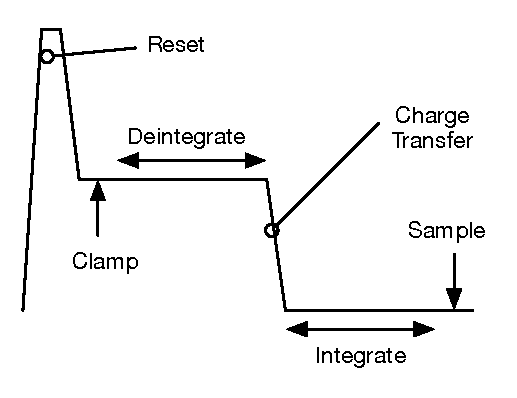
\includegraphics[keepaspectratio=true]{VideoSig.pdf}}
 \caption{Video Signal From CCD}
 \label{VideoSig}
 \end{figure}
Figure \ref{VideoSig} shows voltage versus time for a typical CCD video signal.
\subsection{Building blocks}
\schempage{Chain.1}
\schempage{Chain.2}
\schempage{DrainRegulator}
\schempage{PerChip.1}
\schempage{PerChip.2}
\schempage{PerChip.3}
\schempage{PerChip.4}
\schempage{PerChip.5}
\schempage{PerChip.6}
\schempage{PerChip.7}
\schempage{PerChip.8}
\schempage{Pump}
\subsection{Video Board Top Level}
\schempage{Video.1}
\schempage{Video.2}
\schempage{Video.3}
\schempage{Video.4}
\schempage{Video.5}
\schempage{Video.6}
\schempage{Video.7}
\schempage{Video.8}
\subsection{Video Board Connectors}

J1, J2, J3, and J4 connect to the flexprint cables from CCD1, CCD2, CCD3, and CCD4, respectively. Table \ref{J1} shows the pinout of J1. The -1 at the end of most net names indicates that the net serves CCD1. For J2, the corresponding net names end in -2, etc. Table \ref{J5} shows the pinout for J5, which serves the external temperature sensors and heater. Table \ref{Stack} covers Js, the board stack connector.

\begin{longtable}{|l|l|l|l|}
\caption{Flexprint Connector} \label{J1} \\
\hline
Connector & Pin & Net & Signal \\
\hline \endfirsthead
\caption{Flexprint Connector (continued)} \\
\hline 
Connector & Pin & Net & Signal \\
\hline
\endhead
\hline \endfoot
\input{CCD-51pin.tex}
\end{longtable}


\begin{table}[ht!]
\caption{Temperature Connector}
\begin{tabular}{|l|l|lH|} %Comment column hidden for now
\hline
Connector & Pin & Net & Comment \\
\hline
\input{TempConn.tex}
\hline
\end{tabular}
\label{J5}
\end{table}


\section{Interface Board}
\label{Interface}
\subsection{Building blocks}
\subsubsection{Drivers for high capacitance (parallel) clocks}
\schempage{Booster}
\schempage{ParallelPair}
\schempage{ParallelReg}
\subsubsection{Drivers for low capacitance clocks}
\schempage{SerialDriver}
\schempage{SerialRegulator}
\subsubsection{Clock drivers for one CCD}
\schempage{DriverSet.1}
\schempage{DriverSet.2}
\schempage{DriverSet.3}
\schempage{DriverSet.4}
\subsubsection{Power conditioning}
\schempage{ArtixPower}

Figure \ref{ArtixPower} shows the power regulators for the Artix FPGA. An RC filter on the reference insures that the 1.8V AUX power rises more slowly than the 1V core power. The 2.5V and 3.3V IO power follow the 1.8V AUX power with additional delays. This insures proper initialization. Q5 pulls down the 3.3V IO power if the 1.8V level is low, insuring that the rated maximum 2.625V difference cannot be exceeded for more than the allowed time (see Xilinx data sheet DS181). The resistors on the collectors of the pass transistors limit the surge current, and are rated to handle the fault current if the FPGA should latch up. 
\subsection{Interface Board Top Level}
\schempage{Interface.1}
Figure \ref{Interface.1} shows the Artix FPGA (U4). Its pin connections are too complex to draw: Table \ref{Artix} shows them. J9 is the JTAG header for FPGA debugging. J6 is the data connector to the DHU. J8 is test signals and configuration jumpers for the FPGA. Table \ref{IJ8} shows its pinout. For the pinouts of Js, the stacking connector, see Table \ref{Stack}.


\begin{table}[ht!]
\caption{FPGA Test Header}
\begin{tabular}{|l|l|lH|} %Comment column hidden for now
\hline
Connector & Pin & Net & Comment \\
\hline
\input{Interface.J8.tex}
\hline
\end{tabular}
\label{IJ8}
\end{table}

\begin{longtable}{|Hl|l|l|} %Hide the refdes field
\caption{Artix FPGA Connections} \label{Artix} \\
\hline
Connector & Pin & Net & Signal \\
\hline \endfirsthead
\caption{Artix FPGA Connections (continued)} \\
\hline 
Connector & Pin & Net & Signal \\
\hline
\endhead
\hline \endfoot
\input{Interface.U4.tex}
\end{longtable}

\FloatBarrier
\schempage{Interface.2}
\FloatBarrier
\schempage{Interface.3}
\FloatBarrier
\schempage{Interface.4}
\FloatBarrier
\schempage{Interface.5}
\FloatBarrier
\schempage{Interface.6}
\FloatBarrier
\schempage{Interface.7}
\FloatBarrier
Figure \ref{Interface.7} shows power input from the DHU (J7) and low voltage power conditioning. LEDs are for debugging: we will not install them on flight boards.

\section{Driver Board}
\label{Driver}
See the previous section for the DriverSet building blocks.
\schempage{Driver.1}
\schempage{Driver.2}
\schempage{Driver.3}

\section{Stack Interconnection}

\tiny{
% This is pretty crazy; here's the hack that makes this happen:
% http://tex.stackexchange.com/a/174166
    \begin{longtable}{|m{0.1\textwidth}|m{0.1\textwidth}|m{0.1\textwidth}|m{0.1\textwidth}|m{0.1\textwidth}|m{0.1\textwidth}|m{0.1\textwidth}|m{0.1\textwidth}|@{}m{0pt}@{}}
    \caption{Inter-board Stack Connections} \label{Stack} \\
    \hline
    \input{StackMap.tex}
    \end{longtable}
}

% get back to normal
\normalsize

\section{Operating Parameters and Housekeeping Channels}

While the implementation details differ, the housekeeping channels and the DAC-controlled parameters share a common addressing scheme. An address is seven bits. All seven are provided to the multiplexors and their selection logic as HKA[6:0]. The most significant four bits DCS[3:0] drive the DAC selection logic: the least significant three bits are part of the serial command that sets a DAC. In the following tables CC represents two bits selecting the CCD in offset binary (00$\Rightarrow$CCD1, 01$\Rightarrow$CCD2, 10$\Rightarrow$CCD3, 11$\Rightarrow$CCD4).

The control ranges often go outside the actual range allowed for the parameters, which depend on circuit details and power supply voltages. \textcolor{red}{I will document these limits in the future.} Control is sometimes relative to another parameter. If the control range is not given, the parameter is not under DAC control.
\subsection{Bias Group}
\begin{table}[ht!]
\caption{Bias Group}
\begin{tabular}{|l|l|l|l|}
\hline
\multicolumn{4}{|l|}{Address 0CCXXXX} \\
\hline
XXXX & Housekeeping Signal & Scale & Control Range \\
\hline
0000 & Output Gate & $\pm$16.5V & -8.0V, 4.0V \\
0001 & Input Gate 1 & $\pm$16.5V   & -8.0V, 4.0V \\
0010 & Input Gate 2 & $\pm$16.5V   & -8.0V, 4.0V \\
0011 & Scupper & $\pm$16.5V  & 0, 15.0V \\
0100 & Reset Drain & $\pm$16.5V & 0, 15.0V \\
0101 & Backside & $\pm$16.5V & 0, 5.0V \\
0110 & Substrate & $\pm$82V  & 0, -50V \\
0111 & Board Temperature & $\pm$360K &\\
1000 & Output Drain A & $\pm$27.3V & 0, 10.0V$\dagger$ \\
1001 & Output Drain B & $\pm$27.3V& 0, 10.0V$\dagger$ \\
1010 & Output Drain C & $\pm$27.3V& 0, 10.0V$\dagger$ \\
1011 & Output Drain D & $\pm$27.3V&  0, 10.0V$\dagger$ \\
1100 & Output Source A & $\pm$27.3V &\\
1100 & Output Source B & $\pm$27.3V &\\
1100 & Output Source C & $\pm$27.3V &\\
1100 & Output Source D & $\pm$27.3V &\\
\hline
\end{tabular}
\vspace{5pt}

$\dagger$ Relative to Reset Drain for the specified chip
\label{biastab}
\end{table}

\subsection{Clock Driver Group}
\begin{table}[ht!]
\caption{Clock Driver Group}
\begin{tabular}{|l|l|l|l|}
\hline
\multicolumn{4}{|l|}{Address 10CCXXX} \\
\hline
XXX & Housekeeping Signal & Scale  & Control Range \\
\hline
000 & Parallel High & $\pm$16.5V & 0, 18.1V$\dagger$ \\
001 &Parallel Low &$\pm$16.5V & 0, -13.2V \\
010 & Serial High &$\pm$16.5V & 14.9V, -14.9V \\
011 & Serial Low &$\pm$16.5V & 14.9V, -14.9V \\
100 & Reset High &$\pm$16.5V & 14.9V, -14.9V \\
101 &Reset Low &$\pm$16.5V & 14.9V, -14.9V \\
110 &Input Diode High &$\pm$16.5V & 0, +15.0V \\
111 & Input Diode Low &$\pm$16.5V & 0, +15.0V \\
\hline
\end{tabular}
\vspace{5pt}

$\dagger$ Relative to Parallel Low for the specified chip
\label{clocktab}
\end{table}
\subsection{Heater Group}
\begin{table}[ht!]
\caption{Heater Group}
\begin{tabular}{|l|l|l|l|}
\hline
\multicolumn{4}{|l|}{Address 1100000} \\
\hline
XXX & Housekeeping Signal & Scale &  Control Range \\
\hline
1100000 & Heater Current & $\pm$418mA & 0, 12.5V$\dagger$ \\
\hline
\end{tabular}
\vspace{5pt}

$\dagger$ Control range in mA depends on the external heater resistance
\label{heattab}
\end{table}
\subsection{Interface Group}
\begin{table}[ht!]
\caption{Interface Group}
\begin{tabular}{|l|l|l|}
\hline
\multicolumn{3}{|l|}{Address 1101XXX} \\
\hline
XXX & Housekeeping Signal & Scale  \\
\hline
000 & Board Temperature & $\pm$360K\\
001 & +15 & $\pm$16.5V\\
010 & +5 & $\pm$16.5V\\
011 & -12 & $\pm$16.5V\\
100 & +3.3F & $\pm$16.5V\\
101 & +2.5F & $\pm$16.5V\\
110 & +1.8F & $\pm$16.5V\\
111 & +1F & $\pm$16.5V\\
\hline
\end{tabular}
\label{inttab}
\end{table}
\subsection{Thermal Group}
\begin{table}[ht!]
\caption{Thermal Group}
\begin{tabular}{|l|l|l|}
\hline
\multicolumn{3}{|l|}{Address 111XXXX} \\
\hline
XXX & Housekeeping Signal & Scale  \\
\hline
0000 & Pt1000 sensor 1 & -125C, +130C\\
0001 & Pt1000 sensor 2 & -125C, +130C\\
0010 & Pt1000 sensor 3 & -125C, +130C\\
0011 & Pt1000 sensor 4 & -125C, +130C\\
0100 & Pt1000 sensor 5 & -125C, +130C\\
0101 & Pt1000 sensor 6 & -125C, +130C\\
0110 & Pt1000 sensor 7 & -125C, +130C\\
0111 & Pt1000 sensor 8 & -125C, +130C\\
1000 & Pt1000 sensor 9 & -125C, +130C\\
1001 & Pt1000 sensor 10 & -125C, +130C\\
1010 & Pt1000 sensor 11 & -125C, +130C\\
1011 & Pt1000 sensor 12 & -125C, +130C\\
1100 & AlCu sensor CCD1 & -150C, +40C\\
1101 & AlCu sensor CCD2 & -150C, +40C\\
1110 & AlCu sensor CCD3 & -150C, +40C\\
1111 & AlCu sensor CCD4 & -150C, +40C\\
\hline
\end{tabular}
\label{ttab}
\end{table}

The Thermal Group (Table \ref{ttab}) sensors are external temperature-sensitive resistors. The nominal range for the circuitry is $500\Omega$ to $1500\Omega$, which translates into the given temperature ranges. It may be useful to calibrate the board using external fixed resistors near the limits of the range.

\end{document}
